\documentclass[a4paper]{article}
\usepackage{tikz}
\usetikzlibrary{decorations}
\usetikzlibrary{decorations.pathmorphing, arrows.meta}
\usetikzlibrary{calc}
\usepackage{apacite}
\usepackage{tabularx}
\usepackage{siunitx}
\usepackage{amsmath}
\usepackage{rotating}
\usepackage{colortbl}
\usepackage{multirow}
\usepackage{arydshln} % Dashed hline
\usepackage{makecell} % Makecell
\usepackage{graphicx}
\usepackage[absolute]{textpos}


\begin{document}


\begin{titlepage}
    \title{\textbf{How does the moment of inertia affect the period of Maxwell's Wheel? \\ \small Physics HL Internal Assesment}}
    \author{Zhou Changhui}
    \date{\today}
    \maketitle
    %\tableofcontents
\end{titlepage}

\section{Introduction and background knowledge}

Back in ancient Greece (around 220 B.C.), Archimedes has laid solid foundation for rigid body statics by discovering and formalizing the equilibrium requirement for levers. People studied Archimedes's work and developed concepts like torque after then, but it was not until Issac Newton (1643-1727) formulated Newton's Laws of Motion that humans are well equipped for rigid body dynamics \cite{farber-1961}. With the assistance of advanced mathematical tools, Leonhard Eular (1707-1783) successfully formalized the dynamics of rigid bodies and derived the concepts of moment of inertia and principal axes \cite{marquina2016leonhard}.

Just like inertia (which is determined by mass) in translational motion, the moment of inertia evaluates a body's ability to resist angular acceleration. Generally speaking, the further away the mass is distributed from its axis of rotation, the larger the body's moment of inertia is. Objects with large moment of inertia are good at storing rotational kinetic energy, which makes them suitable for objects like flywheels, while objects with small moment of inertia can rotate faster. 

Maxwell's wheel is commonly used as an instrument to illustrate the conservation of energy and the concept of rotational kinetic energy in physics education. It can also be utilized to measure the moment of inertia of a disk-shaped object. This experiment aims at discovering the significance of the moment of inertia in a Maxwell's wheel experiment.

\textbf{Research question: How does the moment of inertia affect the period of Maxwell's Wheel?}

\section{Hypothesis and reasoning}

\begin{figure}[ht]
    \centering
    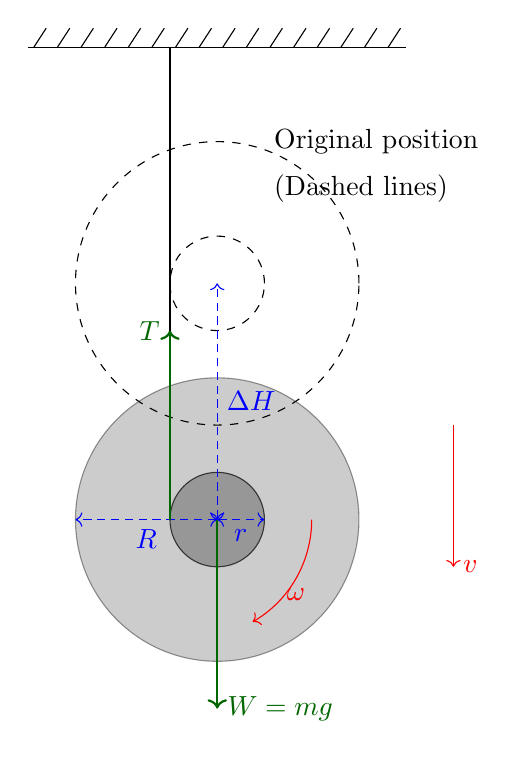
\begin{tikzpicture}[scale = 0.6] % Energy analysis tikzpic 
        \coordinate (O) at (0, 0);
        \draw[fill = gray, opacity = 0.4] (O) circle (3);
        \draw[fill = gray, opacity = 0.7] (O) circle (1);
        \draw[dashed] (0, 5) circle (3);
        \draw[dashed] (0, 5) circle (1);
        \node[right] at (1, 8) {Original position};
        \node[right] at (1, 7) {(Dashed lines)};
        \draw (-4, 10) -- (4, 10);
        \foreach \x in {-3.75, -3.25, ..., 3.75} 
            \draw[xshift = \x cm] (0.13, 10.4) -- (-0.13, 10);
        \draw[thick] (-1, 4) -- (-1, 10); 

        % Lengths
        \draw[<->, densely dashed, blue] (0, 0) -- (1, 0) node[midway, below, scale = 1] {$r$};
        \draw[<->, densely dashed, blue] (0, 0) -- (-3, 0) node[midway, below, scale = 1] {$R$};
        \draw[<->, densely dashed, blue] (0, 0) -- (0, 5) node[midway, right, scale = 1] {$\Delta H$};

        % Kinetics
        \draw[->, red] (5, 2) -- (5, -1) node[right, scale = 1] {$v$};
        \draw[->, red] (2, 0) arc (0: -60: 2.5) node[midway, right, below, scale = 1] {$\omega$};

        % Forces
        \draw[->, black!60!green, thick] (-1, 0) -- (-1, 4) node[above, left, scale = 1] {$T$};
        \draw[->, black!60!green, thick] (0, 0) -- (0, -4) node[below, right, scale = 1] {$W = mg$};
    \end{tikzpicture}
    \caption{Model of a Maxwell's Wheel}
    \label{fig.maxwellwheel}
\end{figure}

As is shown in Figure \ref{fig.maxwellwheel}, the Maxwell's wheel mainly consists of three parts: a wheel of radius $R$, an axle of radius $r$, and a string. Aside from friction, two forces are acting on the pendulum: the tension from the string and the gravitational force. During the entire process, the gravitational potential energy converts to kinetic energy of the wheel. 

The downward movement and the upward movement is basically symmetric, so only the downward reaction needs algebraric analysis.

Since the wheel is not in equilibrium, its hard to analyze the magnitude of tention $T$. However, the problem can be tackled using conservation of energy.

Due to the negeligibility of friction, we can assume that all the gravitational potential energy lost is converted to the kinetic energy. Or more specificly, the sum of the translational kinetic energy and rotational kinetic energy should equal to the loss in gravitational potential energy. Or formally,

\begin{equation}
    mg\Delta h = \frac{1}{2}m v^2 + \frac{1}{2} I \omega ^2
\end{equation}


where $I$ is the moment of inertia of the entire wheel. 

Moreover, using the definition of velocity and angular velocity, the following identites can be derived,

\begin{equation}
    \dfrac{\mathrm{d}\Delta H}{\mathrm{d}t} = v
\end{equation}

\begin{equation}
    \omega r = v
\end{equation}

\begin{equation}
    \Delta H(0) = 0
\end{equation}

Therefore

\begin{equation}
    mg\Delta H = \frac{1}{2}m v^2 + \frac{1}{2} \frac{I}{r^2} v ^2
\end{equation}

After moving and combining the terms

\begin{equation}
    \frac{2mg\Delta H}{m+\frac{I}{r^2}} = (\dfrac{\mathrm{d}\Delta H}{\mathrm{d}t})^2
\end{equation}

Moving ${\mathrm{d}\Delta H}/{\mathrm{d}t}$ to the left size and make its index $1$,

\begin{equation}
    \dfrac{\mathrm{d}\Delta H}{\mathrm{d}t} = \sqrt{\frac{2mg}{m+\frac{I}{r^2}}} \Delta H ^ {0.5}
\end{equation}

This is a simple ODE, with the help of formula (4), we can get that,

\begin{equation}
    \Delta H(t) = \dfrac{mg}{2m+\frac{2I}{r^2}} t^2
\end{equation}

The downward movement terminates when $\Delta H(t) = l$, which means 

\begin{equation}
    t_{down} = \sqrt{\dfrac{(2m+\frac{2I}{r^2})l}{mg}}
\end{equation}

The entire period of the Maxwell's Wheel is 

\begin{equation}
    T = 2t_{down} = 2\sqrt{\dfrac{(2m+\frac{2I}{r^2})l}{mg}}
\end{equation}

which can be re-written as 

\begin{equation}
    T^2 = 8l\dfrac{(m+\frac{I}{r^2})}{mg}
\end{equation}

Or

\begin{equation}
    T^2 = \dfrac{8l}{mgr^2} I + \dfrac{8l}{g}
\end{equation}

From this formula, the hypothesis can be derived: \textbf{$T$ increases as $I$ increases. $T^2$ and $I$ has a linear relationship.}

\section{Experiment design}

\subsection{Variables} 

\begin{itemize}
    \item Independent variable: Moment of inertia (manipulated by changing the distance from the magnets to the pivot: $r' = 2.5, 3.5, 4.5, 5.5, 6.5, 7.5, 8.5 \SI{}{cm}$).
    \item Dependent variable: ``Period'' of the Maxwell's Wheel (Time between two lowest positions).
    \item Controlled variables: The material, mass and size of the plate and magnets. The length of the string. The mass, radius and length of the axle, etc.
\end{itemize}

Independent variable turned out to be $0.668, 0.776, 0.919, 1.09, 1.31, 1.56$ and $1.85 \times 10^{-3}\SI{}{kgm^2}$ (as is shown in Section \ref{sec.results}). The independent variable is hard to manipulate, as the moment of inertia results from the arithmatical addition of two parts: the acrylic disk and the magnets. The former part is independent of $r'$, making it impossibe to reach very small $r'$. The latter part is proportional to $r'^2$, resulting in difficulty to place the magnets on the acrylic plane if even distribution between $I$ is needed. 

Controlled variable table TBD.

\subsection{Materials}

\begin{itemize}
    \item[*] 2 Iron stands (height $\approx \SI{50}{cm}$)
    \item[*] 2 Cotton strings (length $\approx \SI{70}{cm}$)
    \item[*] 1 Acrylic disc (radius $\approx \SI{10}{cm}$, mass $\approx \SI{110}{g}$)
    \item[*] 16 Magnets (radius $\approx \SI{3.0}{cm}$, mass $\approx \SI{23}{g}$)
    \item[*] 1 Force gauge ($\SI{50}{N}$)
    \item[*] 1 Tape rule
    \item[*] 1 Electric balance
    \item[*] 1 Vernier caliper
    \item[*] 1 Hot glue gun  
\end{itemize}

\subsection{Setup diagram}

The apparatus is set up by hanging the Maxwell's Wheel between two iron stands using cotton string, as is shown in Figure \ref{fig.setupdiagram}.

\begin{figure}[ht]
    \centering
    
    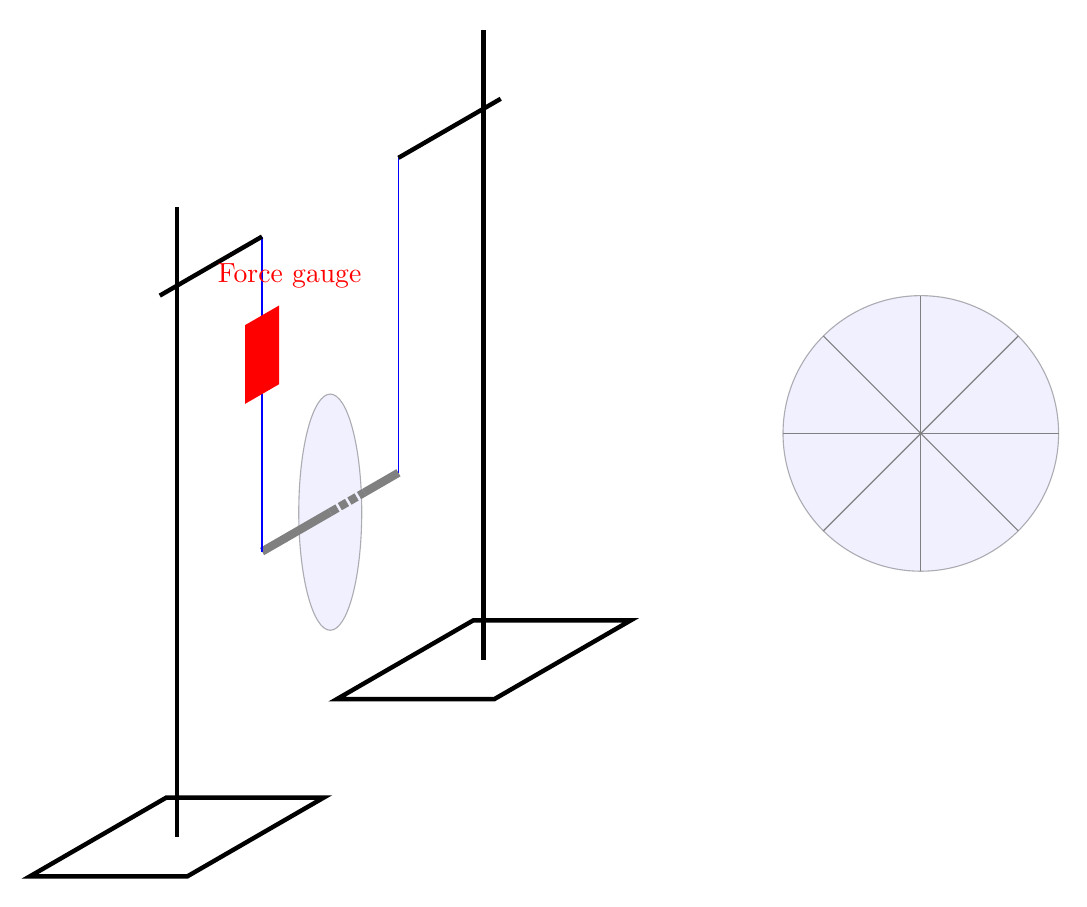
\begin{tikzpicture}[scale = 0.5]
    % No I think this is stupid
    
    % The acrylic plate 
        \draw[fill=blue!20, opacity=0.3, even odd rule] (0,0) ellipse (0.8 and 3);
        \coordinate (P) at ($(0,0) - (30:2)$);
        \coordinate (Q) at ($(0,0) + (30:2)$);
        \draw[line width=3pt, gray] (P) -- (0,0);
        \draw[densely dotted, line width = 3pt, gray] (0,0) -- ($(0,0) + (30:1)$);
        \draw[line width=3pt, gray] ($(0,0) + (30:1)$) -- (Q);
        \draw[blue, semithick] (P) -- ($(P) + (0, 8)$);
        \draw[blue, semithick] (Q) -- ($(Q) + (0, 8)$);
        \draw[black, ultra thick] ($(P) + (0, 8)$) -- ($(P) + (0, 8) - (30:3)$);
        \draw[black, ultra thick] ($(Q) + (0, 8)$) -- ($(Q) + (0, 8) + (30:3)$);
        \coordinate (R) at ($(P) + (0, -6) - (30:2.5)$);
        \coordinate (S) at ($(Q) + (0, -6) + (30:2.5)$);
        \draw[black, ultra thick] ($(P) + (0, 10) - (30:2.5)$) -- (R);
        \draw[black, ultra thick] ($(Q) + (0, 10) + (30:2.5)$) -- (S);
        \draw[black, ultra thick] ($(R) + (30: 2) + (2, 0)$) -- ($(R) + (30: 2) - (2, 0)$) -- ($(R) - (30: 2) - (2, 0)$) -- ($(R) - (30: 2) + (2, 0)$) -- cycle;
        \draw[black, ultra thick] ($(S) + (30: 2) + (2, 0)$) -- ($(S) + (30: 2) - (2, 0)$) -- ($(S) - (30: 2) - (2, 0)$) -- ($(S) - (30: 2) + (2, 0)$) -- cycle;
        \coordinate (X) at ($(P) + (0, 5)$);
        \fill[red] ($(X) + (0, 1) + (30: 0.5)$) -- ($(X) + (0, 1) - (30: 0.5)$) -- ($(X) - (0, 1) - (30: 0.5)$) -- ($(X) - (0, 1) + (30: 0.5)$) -- cycle;
        \node[red] at ($(X) + (0.7, 2)$) {Force gauge};
        
        \coordinate (O) at (15, 2);
        \draw[fill=blue!20, opacity=0.3] (O) circle (3.5);
        \draw[gray] ($(O) - (0 : 3.5)$) -- ($(O) + (0 : 3.5)$);
        \draw[gray] ($(O) - (45 : 3.5)$) -- ($(O) + (45 : 3.5)$);
        \draw[gray] ($(O) - (90 : 3.5)$) -- ($(O) + (90 : 3.5)$);
        \draw[gray] ($(O) - (135 : 3.5)$) -- ($(O) + (135 : 3.5)$);
        %\draw[black, ultra thick]
    \end{tikzpicture}
    \caption{Setup diagram}
    \label{fig.setupdiagram}
\end{figure}

\subsection{Procedure}

\begin{enumerate}
    \item Measure the total mass of the magnets, mass of the acrylic plate, radius of the acrylic plate, radius of the axle and maximum vertical displacement after setting up the apparatus as is shown in Figure \ref{fig.setupdiagram}
    \item Find a pair of diameters of the acrylic plane that is perpendicular to each other. This can be done by drawing the perpendicular bisector of an arbitrary pair of perpendicular chords. 
    \item Calibrate both axis with the assistance of a ruler. Make sure the center of the circle is scaled zero. 
    \item Attach four pairs of magnets to the plane.
    \item Adjust the position of the magnets to make the distance for the magnets' centers of mass are $r = \SI{8.5}{cm}$. This can be done by placing the magnet (with radius $r' = \SI{3}{cm}$) between $r = \SI{10}{cm}$ mark and $r = \SI{7}{cm}$ mark, while touching the both marks.
    \item Fix the magnets with glue guns.
    \item Swirl up the axle until it reaches the designated point, start the forcemeter and release the wheel. 
    \item Record the time for the first and second time where the forcemeter reading reaches local maxima \footnote{This is done with the assistance of a program. If the first local maximum is not prominant, the second and the third local maxima is used instead.} 
    \item Repeat Steps 7 and 8 for $4$ additional trials.
    \item Repeat Steps 5 to 9 with $r = 7.5, 6.5, 5.5, 4.5, 3.5 \SI{}{cm}$.
\end{enumerate}

\section{Results}
\label{sec.results}

\subsection{Raw data}

Raw data is collected as follows:

\begin{itemize}
    \item Total mass of the magnets $M_m$ : $193.70\pm0.01\SI{}{g}$
    \item Total mass of the acrylic plate $M_a$: $193.17\pm0.01\SI{}{g}$
    \item Radius of the acrylic plate $R_a$: $10.0\pm0.05\SI{}{cm}$
    \item Radius of the axle $r$: $4.0\pm0.1\SI{}{mm}$
    \item Maximum vertical displacement $H$: $20\pm0.5\SI{}{cm}$
    \item Other data is shown in Table \ref{tab.raw}.
\end{itemize}



\begin{table}[ht]
\centering
\caption{Raw Data}
\label{tab.raw}
\begin{tabularx}{\textwidth}{XXXXXXXXXX}
\hline
\hline
\multicolumn{5}{c}{Experiments 1-4} & \multicolumn{5}{c}{Experiments 5-7} \\
\hline
No.         & \makecell{$r(\SI{}{cm})$ \\ $\pm \SI{0.1}{cm}$ }  & Trial & \makecell{$t_1(\SI{}{s})$ \\ $\pm \SI{0.01}{s}$ } & \makecell{$t_2(\SI{}{s})$ \\ $\pm \SI{0.01}{s}$ } & 
No.         & \makecell{$r(\SI{}{cm})$ \\ $\pm \SI{0.1}{cm}$ }  & Trial & \makecell{$t_1(\SI{}{s})$ \\ $\pm \SI{0.01}{s}$ } & \makecell{$t_2(\SI{}{s})$ \\ $\pm \SI{0.01}{s}$ } \\
\hline
\multirow{5}{*}{1} & \multirow{5}{*}{$2.5$} & 1     & $2.28$   & $6.68$   & 
\multirow{5}{*}{5} & \multirow{5}{*}{$6.5$} & 1     & $3.58$   & $9.48$   \\
                   &                                & 2     & $2.25$   & $6.63$   &
                   &                                & 2     & $9.28$   & $15.23$  \\
                   &                                & 3     & $2.48$   & $7.03$   &
                   &                                & 3     & $3.45$   & $9.48$   \\
                   &                                & 4     & $6.73$   & $11.28$  &
                   &                                & 4     & $3.53$   & $9.43$   \\
                   &                                & 5     & $2.33$   & $6.78$   &
                   &                                & 5     & $9.28$   & $15.23$   \\
\cdashline{1-5} \cdashline{6-10}
\multirow{5}{*}{2} & \multirow{5}{*}{$3.5$} & 1     & $2.73$   & $7.23$   & 
\multirow{5}{*}{6} & \multirow{5}{*}{$7.5$} & 1     & $10.43$  & $17.68$  \\
                   &                                & 2     & $7.03$   & $11.53$  &
                   &                                & 2     & $3.93$   & $10.68$  \\
                   &                                & 3     & $2.78$   & $7.63$   &
                   &                                & 3     & $4.08$   & $11.03$  \\
                   &                                & 4     & $2.58$   & $7.38$   &
                   &                                & 4     & $4.23$   & $11.13$  \\
                   &                                & 5     & $2.83$   & $7.33$   &
                   &                                & 5     & $4.03$   & $10.53$   \\
\cdashline{1-5} \cdashline{6-10}
\multirow{5}{*}{3} & \multirow{5}{*}{$4.5$} & 1     & $2.88$   & $8.13$   & 
\multirow{6}{*}{7} & \multirow{6}{*}{$8.5$} & 1     & $4.08$   & $11.78$  \\
                   &                                & 2     & $3.18$   & $8.63$   &
                   &                                & 2     & $11.68$  & $18.33$  \\
                   &                                & 3     & $3.08$   & $8.53$   &
                   &                                & 3     & $11.48$  & $18.38$  \\
                   &                                & 4     & $2.88$   & $7.88$   &
                   &                                & 4     & $12.03$  & $20.58$  \\
                   &                                & 5     & $3.03$   & $8.28$   &
                   &                                & 5     & $11.78$  & $18.63$   \\
\cdashline{1-5}
\multirow{5}{*}{4} & \multirow{5}{*}{$5.5$} & 1     & $3.28$   & $8.93$   &
                   &                                & 6     & $4.13$   & $11.63$   \\
\cdashline{6-10}
                   &                                & 2     & $3.23$   & $8.73$   & & & & & \\
                   &                                & 3     & $3.23$   & $8.83$   & & & & & \\
                   &                                & 4     & $3.18$   & $8.73$   & & & & & \\
                   &                                & 5     & $3.48$   & $9.23$   & & & & & \\
%\cdashline{1-5}
\hline
\hline
\end{tabularx}
\end{table}

\subsection{Processed data}
\label{sec.procd}

\begin{table}[ht]
\centering
\caption{Processed data}
\label{tab.proc}
\begin{tabular}{lll}
\hline \hline
Experiment & $I(\times 10^{-3}\SI{}{kgm^2})$ & $T^2(\SI{}{s^2})$ \\ \hline
1          & $0.668\pm 0.0201$               & $19.9\pm0.759$    \\
2          & $0.776\pm 0.0237$               & $21.4\pm1.62$     \\
3          & $0.919\pm 0.0528$               & $27.9\pm2.38$     \\
4          & $1.09\pm 0.0309$                & $31.5\pm1.40$     \\
5          & $1.31\pm 0.0345$                & $35.4\pm0.773$    \\
6          & $1.56\pm 0.0381$                & $47.2\pm5.15$     \\
7          & $1.85\pm 0.0417$                & $50.7\pm7.48$     \\ \hline \hline
\end{tabular}
\end{table}

\begin{figure}[ht]
    \centering
    \includegraphics[width = 0.8\textwidth]{grapha.png}
    \caption{$T^2 - I$ graph}
    \label{fig.processedd}
\end{figure}

\subsection{Sample processing}

\section{Discussion and conclusion}

The diagram shows strong correlation between $T^2$ and $I$. The best fit line of $T^2 - I$ has 

\begin{itemize}
    \item a gradient of $(27.3150 \pm 6.9556) \times 10^3\ \SI{}{s^2kg^{-1}m^{-2}}$.
    \item a y-intercept of $1.4557 \SI{}{s^2}$.
\end{itemize}

As is mentioned in Section \ref{sec.procd}, the graph is expected to be a straight line very close to the origin. The diagram shows a graph with relatively small error, supporting the initial hypothesis.

The y-intercept is expected to be $\frac{8l}{mgr^2} \approx 0.16\SI{}{s^2}$, but $1.4557\SI{}{s^2}$ is found. This is almost $9$ times the theoretical value. However, considering the large value of $T$ in data, $1.4557\SI{}{s^2}$ is still less than $10\%$ of the minimum dependent variable. This means it can still be considered an error, whose cause will be discussed in Section \ref{sec.eval}.

The gradient is expected to be $\frac{8l}{g} = 26.3900 \times 10^3\ \SI{}{s^2kg^{-1}m^{-2}}$, where $l$ is the length for lifting (controlled to be close to $\SI{20}{cm}$)and $g$ is the gravitational acceleration near sea level. There is a small $3.51\%$ error between the actual gradient and predicted gradient, and the predicted gradient lies within the uncertainty range of the gradient. The low error shows high accuracy and precision of this experiment.

Error bars are small when $I$ is small, but becomes larger as $I$ gets larger. That might result from the significant horizontal perturbation get greater as $I$ increases. Horizontal movements make the wheel start to swing like a pendulum and makes the motion more chaotic and less trackable. 

The best fit line fails to pass through the fifth error bar, which is also coincidentially a very small error bar. That might result form coincidence, since there is only five trials in each group.

\section{Evaluation}
\label{sec.eval}

The experiment was conducted successfully, gathering sufficient data and supporting the initial hypothesis. However, there are some uncertainties in the experiment that can be improved. 

\begin{itemize}
    \item \textbf{Defect in modelling} It is assumed in the hypothesis that the wheel do not swing horizontally and the string is always vertical, but small horizontal movement is inevitable during the experiment process.
    \item \textbf{Screw-threaded axle} For an ideal Maxwell's Wheel, the radius of the small axle should be constant. However, a screw-threaded axle is utilized to ensure better installation of the wheel, making the string swirl around the thread with inconsistant radius. This can be improved by using an axle that has screw thread only in the middle point. 
    \item \textbf{String attaching} When attaching the wire to the axle, some adhesive (hot glue) is used to ensure connection stability. This also contributed to inconsistant radius. Opt for an axle with a hole for attachment to avoid the use of hot-melt adhesive. 
    \item \textbf{Horizontal movement} The hypothesis is based on negeligibile horizontal movement, but in the real experiment horizontal movement is inevitable because the wheel is controlled and released by hand. Using a plumb line to adjust the string before releasing can minimize the horizontal deflection.
\end{itemize}

\bibliographystyle{apacite}
\bibliography{cit.bib}

\end{document}